\chapter{Avaliação e resultados}\label{Cap:Evaluation}

Para otimizar o streaming de vídeo esférico é essencial conhecer suas principais características que afetam seu desempenho e sua qualidade. Para caracterizar o tráfego de vídeo panorâmico de 360 graus ladrilhado com DASH-SRD, é essencial replicar as condições de transmissão, codificação e segmentação do vídeo durante uma seção do cliente. Além disso, as métricas de avaliação devem ser relacionadas a experiência do usuário e do servidor. Para o cliente o queremos medir o tempo de decodificação, a taxa de bits e a qualidade do vídeo exibido no viewport. Para o servidor, queremos que a melhor qualidade seja entregue com a menor taxa de bits possível e para isso avaliamos métricas de qualidade de codificação tradicional e de vídeo esférico e sua correlação com o a taxa de bits.

Em um sistema de streaming adaptativo como DASH, os chunks do vídeo devem ser codificado de forma que possa ser decodificado de forma independente do chunk anterior, isto é, não tenham dependência temporal. Para isso, o GOP (\textit{Group of pictures}) usado em codificação preditiva, precisa ser do tipo fechado e com o numero de quadros fixo igual a duração do \textit{chunks}. Além disso, para evitar que haja artefatos nas bordas dos ladrilhos durante a reprodução, os ladrilhos precisam ser codificados de forma que a qualidade seja aproximadamente a mesma entre todos os ladrilhos de um quadro ao longo de sua reprodução. Geralmente os vídeos que serão transmitidos devem ser codificados baseado em taxa média para que o buffer de reprodução possa ser facilmente modelado. Porém, se o vídeo for segmentado em ladrilhos, cada ladrilho possuirá uma complexidade diferente, por exemplo, ladrilhos que mapeiam o topo ou a base da esfera tendem a retratar o chão ou o céu, que possuem poucos detalhes, sendo assim a compressão é alta, mesmo usando pouca quantização. Por outro ladro, ladrilhos que mapeiam regiões da esfera com alta atividade temporal e espacial, como movimento, pessoas, texturas, etc, tentem a ser difícil de comprimir. Assim, os ladrilhos de um vídeos não devem possuir a mesma taxa de bit, mas sim a mesma distorção de codificação. Em contra partida, a taxa de bits poderá variar muito dependendo do conteúdo do vídeo, inserindo mais complexidade na modelagem do buffer de reprodução.


\section{Caracterização dos elementos do servidor}

O fluxo de trabalho da caracterização é visto na figura~\ref{fig:fluxograma1}. Os vídeos selecionados São os mesmos empregados no estudo de Nasrabadi~\cite{Nasrabadi2019}. Seis vídeos foram gravados pessoalmente pelo autor em projeção equirretangular. Os demais vídeos foram obtidos do YouTube em projeção cúbica. O processo de download foi executado usando a ferramenta JDownloader\footnote{https://jdownloader.org/} e, devido a variabilidade de qualidades e formatos abrangendo da plataforma, demos preferência a vídeos codificados com h.264, resolução de 4K e 30 fps (quadros por segundo). Apesar disto, os vídeos estavam em duas projeções diferentes e possuíam grande variabilidade de resoluções e taxas de quadro. Isto nos levou a padronizá-los afim de podermos comparar suas características. 

\begin{figure}
    \centering
    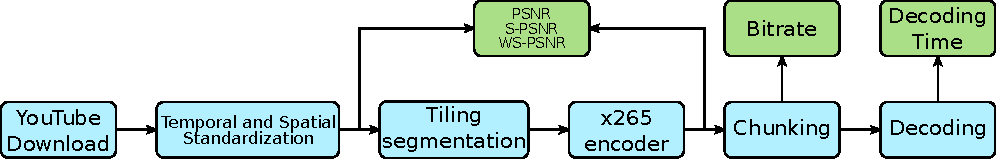
\includegraphics[width=0.7\linewidth]{fig/Fluxograma1}
    \caption{Fluxograma para captura de métricas de desempenho.}
    \label{fig:fluxograma1}
\end{figure}

Assim, topos os vídeos foram convertidos para as projeções cubemap e equirretangular usando o codificador de referência HM 16.9 com a biblioteca 360lib da MPEG\footnote{https://jvet.hhi.fraunhofer. de/svn/svn\_360Lib/}. Em seguida, convertidos para as resoluções $3240\times2160$ (CMP) e $4320\times2160$ (ERP), com taxa de quadros igual a 30 fps. A proporção da projeção foi definida dependendo da projeção utilizada. Para a projeção equirretangular, a proporção é de 2:1, pois ela mapeia os 360° em torno da esfera e os 180° de polo a polo. Já a projeção cúbica apresenta uma proporção de 3:2, pois cada uma das seis faces do cubo é projetada a 90° tanto na latitude quanto na longitude. Por questões práticas, os vídeos foram comprimidos sem perda usando codificador x265 do ffmpeg com CRF igual a 0 e armazenados em arquivos mp4.

A Tabela~\ref{tab:list_videos} exibe a lista dos cinquenta e seis vídeos utilizados. Os vídeos estão codificados com CRF 28 com a configuração padrão do codificador x265. Conforme estudo de Nasrabadi, os vídeos foram classificados de acordo com o movimento da câmera e o numero de objetos na cena. O número de objetos na cena foram definidos pelo autor. O valor da coluna "Grupo" é composto pela primeira inicial do tipo de movimento de câmera (fixo, horizontal, vertical, rotacional, múltiplo) e numero de objetos na cena (nenhum, simples, múltiplo). Assim, o grupo "VM" corresponde ao movimento Vertical com Múltiplos objetos.

\begin{longtable}{|c|c|c|c|c|c|}
\caption{Vídeos usados no experimento}
\label{tab:list_videos} 
\\

\hline
Grupo & Nome & Projeção & SI & TI  &  \makecell{Taxa de \\ Bits (Mbps)} \\
\hline
\endfirsthead

\multicolumn{6}{c}%
{{\bfseries \tablename\ \thetable{} -- Continuação da página anterior}} \\
\hline
Grupo & Nome & Projeção & SI & TI  &  \makecell{Taxa de \\ Bits (Mbps)} \\
\hline

\endhead

\multicolumn{6}{|r|}{{Continua na próxima página}} \\ \hline
\endfoot

\hline
\endlastfoot


\multirow{4}{*}{FN} & \multirow{2}{*}{montana} & ERP &  33.4 &   0.34 &   3.033 \\  \cline{3-6}
                          &                    & CMP &  35.7 &   0.19 &   2.811 \\  \cline{2-6}
   & \multirow{2}{*}{sunset}                   & ERP &  15.6 &   0.44 &   1.571 \\ \cline{3-6}
                          &                    & CMP &  18.7 &   0.46 &   1.442 \\ \hline
                          
\multirow{4}{*}{FS} & \multirow{2}{*}{closet\_tour} & ERP &  51.0 &   1.65 &   2.349 \\ \cline{3-6}
                          &                         & CMP &  57.2 &   1.95 &   2.276 \\ \cline{2-6}
   & \multirow{2}{*}{video\_04}                     & ERP &  49.9 &   1.19 &   2.875 \\ \cline{3-6}
                           &                        & CMP &  50.9 &   1.11 &   2.245 \\ \hline

\pagebreak \hline
\multirow{4}{*}{FM} & \multirow{2}{*}{dubstep\_dance}   & ERP &  32.9 &   6.14 &   2.771 \\ \cline{3-6}
                             &                          & CMP &  38.0 &   6.28 &   2.516 \\ \cline{2-6}
   & \multirow{2}{*}{rhinos}                            & ERP &  38.5 &   0.71 &   3.799 \\ \cline{3-6}
                                    &                   & CMP &  39.8 &   0.63 &   3.251 \\ \hline
                                    
\multirow{4}{*}{HN} & \multirow{2}{*}{drone\_footage}   & ERP &  30.3 &   5.49 &   5.153 \\ \cline{3-6}
                             &                          & CMP &  37.2 &   5.80 &   4.334 \\ \cline{2-6}
   & \multirow{2}{*}{petite\_anse}                      & ERP &  41.4 &   7.84 &   5.913 \\ \cline{3-6}
                             &                          & CMP &  39.4 &   7.50 &   4.919 \\ \hline
                             
\multirow{4}{*}{HS} & \multirow{2}{*}{cable\_cam}   & ERP &  49.7 &  17.54 &  18.790 \\ \cline{3-6}
                             &                      & CMP &  53.1 &  18.47 &  17.554 \\ \cline{2-6}
   & \multirow{2}{*}{motorsports\_park}             & ERP &  35.6 &   8.15 &   3.545 \\ \cline{3-6}
                             &                      & CMP &  41.7 &   8.88 &   3.413 \\ \hline
                             
\multirow{4}{*}{HM} & \multirow{2}{*}{chariot\_race}    & ERP &  39.1 &  16.87 &   8.034 \\ \cline{3-6}
                             &                          & CMP &  44.8 &  18.99 &   7.519 \\ \cline{2-6}
   & \multirow{2}{*}{nyc\_drive}                        & ERP &  82.7 &  24.59 &  12.176 \\ \cline{3-6}
                             &                          & CMP &  92.7 &  27.72 &  11.565 \\ \hline
                             
\multirow{4}{*}{VN} & \multirow{2}{*}{elevator\_lift}   & ERP &  52.9 &   8.46 &   2.325 \\ \cline{3-6}
                             &                          & CMP &  60.3 &   9.59 &   2.100 \\ \cline{2-6}
   & \multirow{2}{*}{glass\_elevator}                   & ERP &  74.6 &   9.08 &   5.432 \\ \cline{3-6}
                             &                          & CMP &  82.1 &  11.82 &   5.974 \\ \hline
                             
\multirow{4}{*}{VM} & \multirow{2}{*}{drone\_video} & ERP &  77.0 &  15.73 &   7.831 \\ \cline{3-6}
                             &                      & CMP &  84.5 &  18.58 &   7.431 \\ \cline{2-6}
   & \multirow{2}{*}{drop\_tower}                   & ERP &  41.0 &   4.95 &   3.141 \\ \cline{3-6}
                             &                      & CMP &  45.0 &   4.27 &   2.839 \\ \hline
                             
\multirow{4}{*}{RN} & \multirow{2}{*}{video\_19}    & ERP &  44.7 &   7.80 &   1.310 \\ \cline{3-6}
                             &                      & CMP &  48.8 &   9.01 &   1.645 \\ \cline{2-6}
   & \multirow{2}{*}{video\_20}                     & ERP &  31.8 &   5.36 &   0.787 \\ \cline{3-6}
                             &                      & CMP &  36.8 &   6.03 &   0.925 \\ \hline
                             
\multirow{4}{*}{RS} & \multirow{2}{*}{penthouse}    & ERP &  42.2 &   1.56 &   1.421 \\ \cline{3-6}
                             &                      & CMP &  48.3 &   1.61 &   1.458 \\ \cline{2-6}
   & \multirow{2}{*}{video\_22}                     & ERP &  34.7 &   5.59 &   1.055 \\ \cline{3-6}
                             &                      & CMP &  40.6 &   6.56 &   1.166 \\ \hline
                             
\multirow{4}{*}{RM} & \multirow{2}{*}{video\_23}    & ERP &  45.6 &  10.95 &   3.398 \\ \cline{3-6}
                             &                      & CMP &  49.7 &  12.28 &   3.231 \\ \cline{2-6}
   & \multirow{2}{*}{video\_24}                     & ERP &  41.8 &   9.43 &   1.802 \\ \cline{3-6}
                             &                      & CMP &  48.7 &  11.11 &   2.097 \\ \hline
                             
\multirow{4}{*}{MN} & \multirow{2}{*}{angel\_falls} & ERP &  24.3 &   1.89 &   2.690 \\ \cline{3-6}
                             &                      & CMP &  24.2 &   1.95 &   2.233 \\\cline{2-6}
   & \multirow{2}{*}{three\_peaks}                  & ERP &  25.9 &   3.30 &   1.693 \\ \cline{3-6}
                             &                      & CMP &  30.4 &   3.06 &   1.473 \\ \hline
                             
\multirow{4}{*}{MS} & \multirow{2}{*}{drone\_chases\_car}   & ERP &  28.9 &  12.10 &   5.839 \\ \cline{3-6}
                             &                              & CMP &  29.6 &  13.12 &   5.251 \\ \cline{2-6}
   & \multirow{2}{*}{wingsuit\_dubai}                       & ERP &  68.8 &  18.98 &  10.012 \\ \cline{3-6}
                             &                              & CMP &  66.8 &  16.86 &   7.881 \\ \hline
                             

\pagebreak \hline
\multirow{4}{*}{MM} & \multirow{2}{*}{blue\_angels} & ERP &  41.2 &   6.65 &   3.766 \\ \cline{3-6}
                             &                      & CMP &  42.7 &   6.94 &   3.520 \\ \cline{2-6}
   & \multirow{2}{*}{pac\_man}                      & ERP &  23.2 &   6.36 &   1.262 \\ \cline{3-6}
                             &                      & CMP &  28.4 &   7.14 &   1.193 \\
\end{longtable}


As colunas "SI" e "TI" mostram informações espaciais (SI) e temporais (TI), calculadas seguindo a recomendação ITU-T P.910, porém, utilizando a mediana em vez do valor máximo, pois os vídeos são longos e possuem picos que não caracterizam o vídeo em si. Os índices de correlação de Pearson entre SI e taxa de bits, assim como entre TI e taxa de bits, são respectivamente de 0.519 e 0.759 para projeção cúbica e 0,528 e 0,773 para projeção equirretangular, indicando uma influência razoável tanto de SI quanto de TI na taxa de bits, com ênfase à atividade temporal.

Examinando o gráfico de dispersão de SI e TI na Figura~\ref{fig:scatter_si_ti}, observamos um padrão bem distribuído entre os vídeos: a taxa de bits média é de 4,22 Mbps, o SI médio é de 46,3 e o TI médio é de 8,5.  Os índices de correlação de Pearson entre SI e taxa de bits, bem como entre TI e taxa de bits, são de 0.530 e 0.765, respectivamente, significando uma influência razoável tanto de SI quanto de TI na taxa de bits. 

\begin{figure}[h]
\centering
\subfigure[Projeção CMP. \label{fig:scatter_CMP}]{
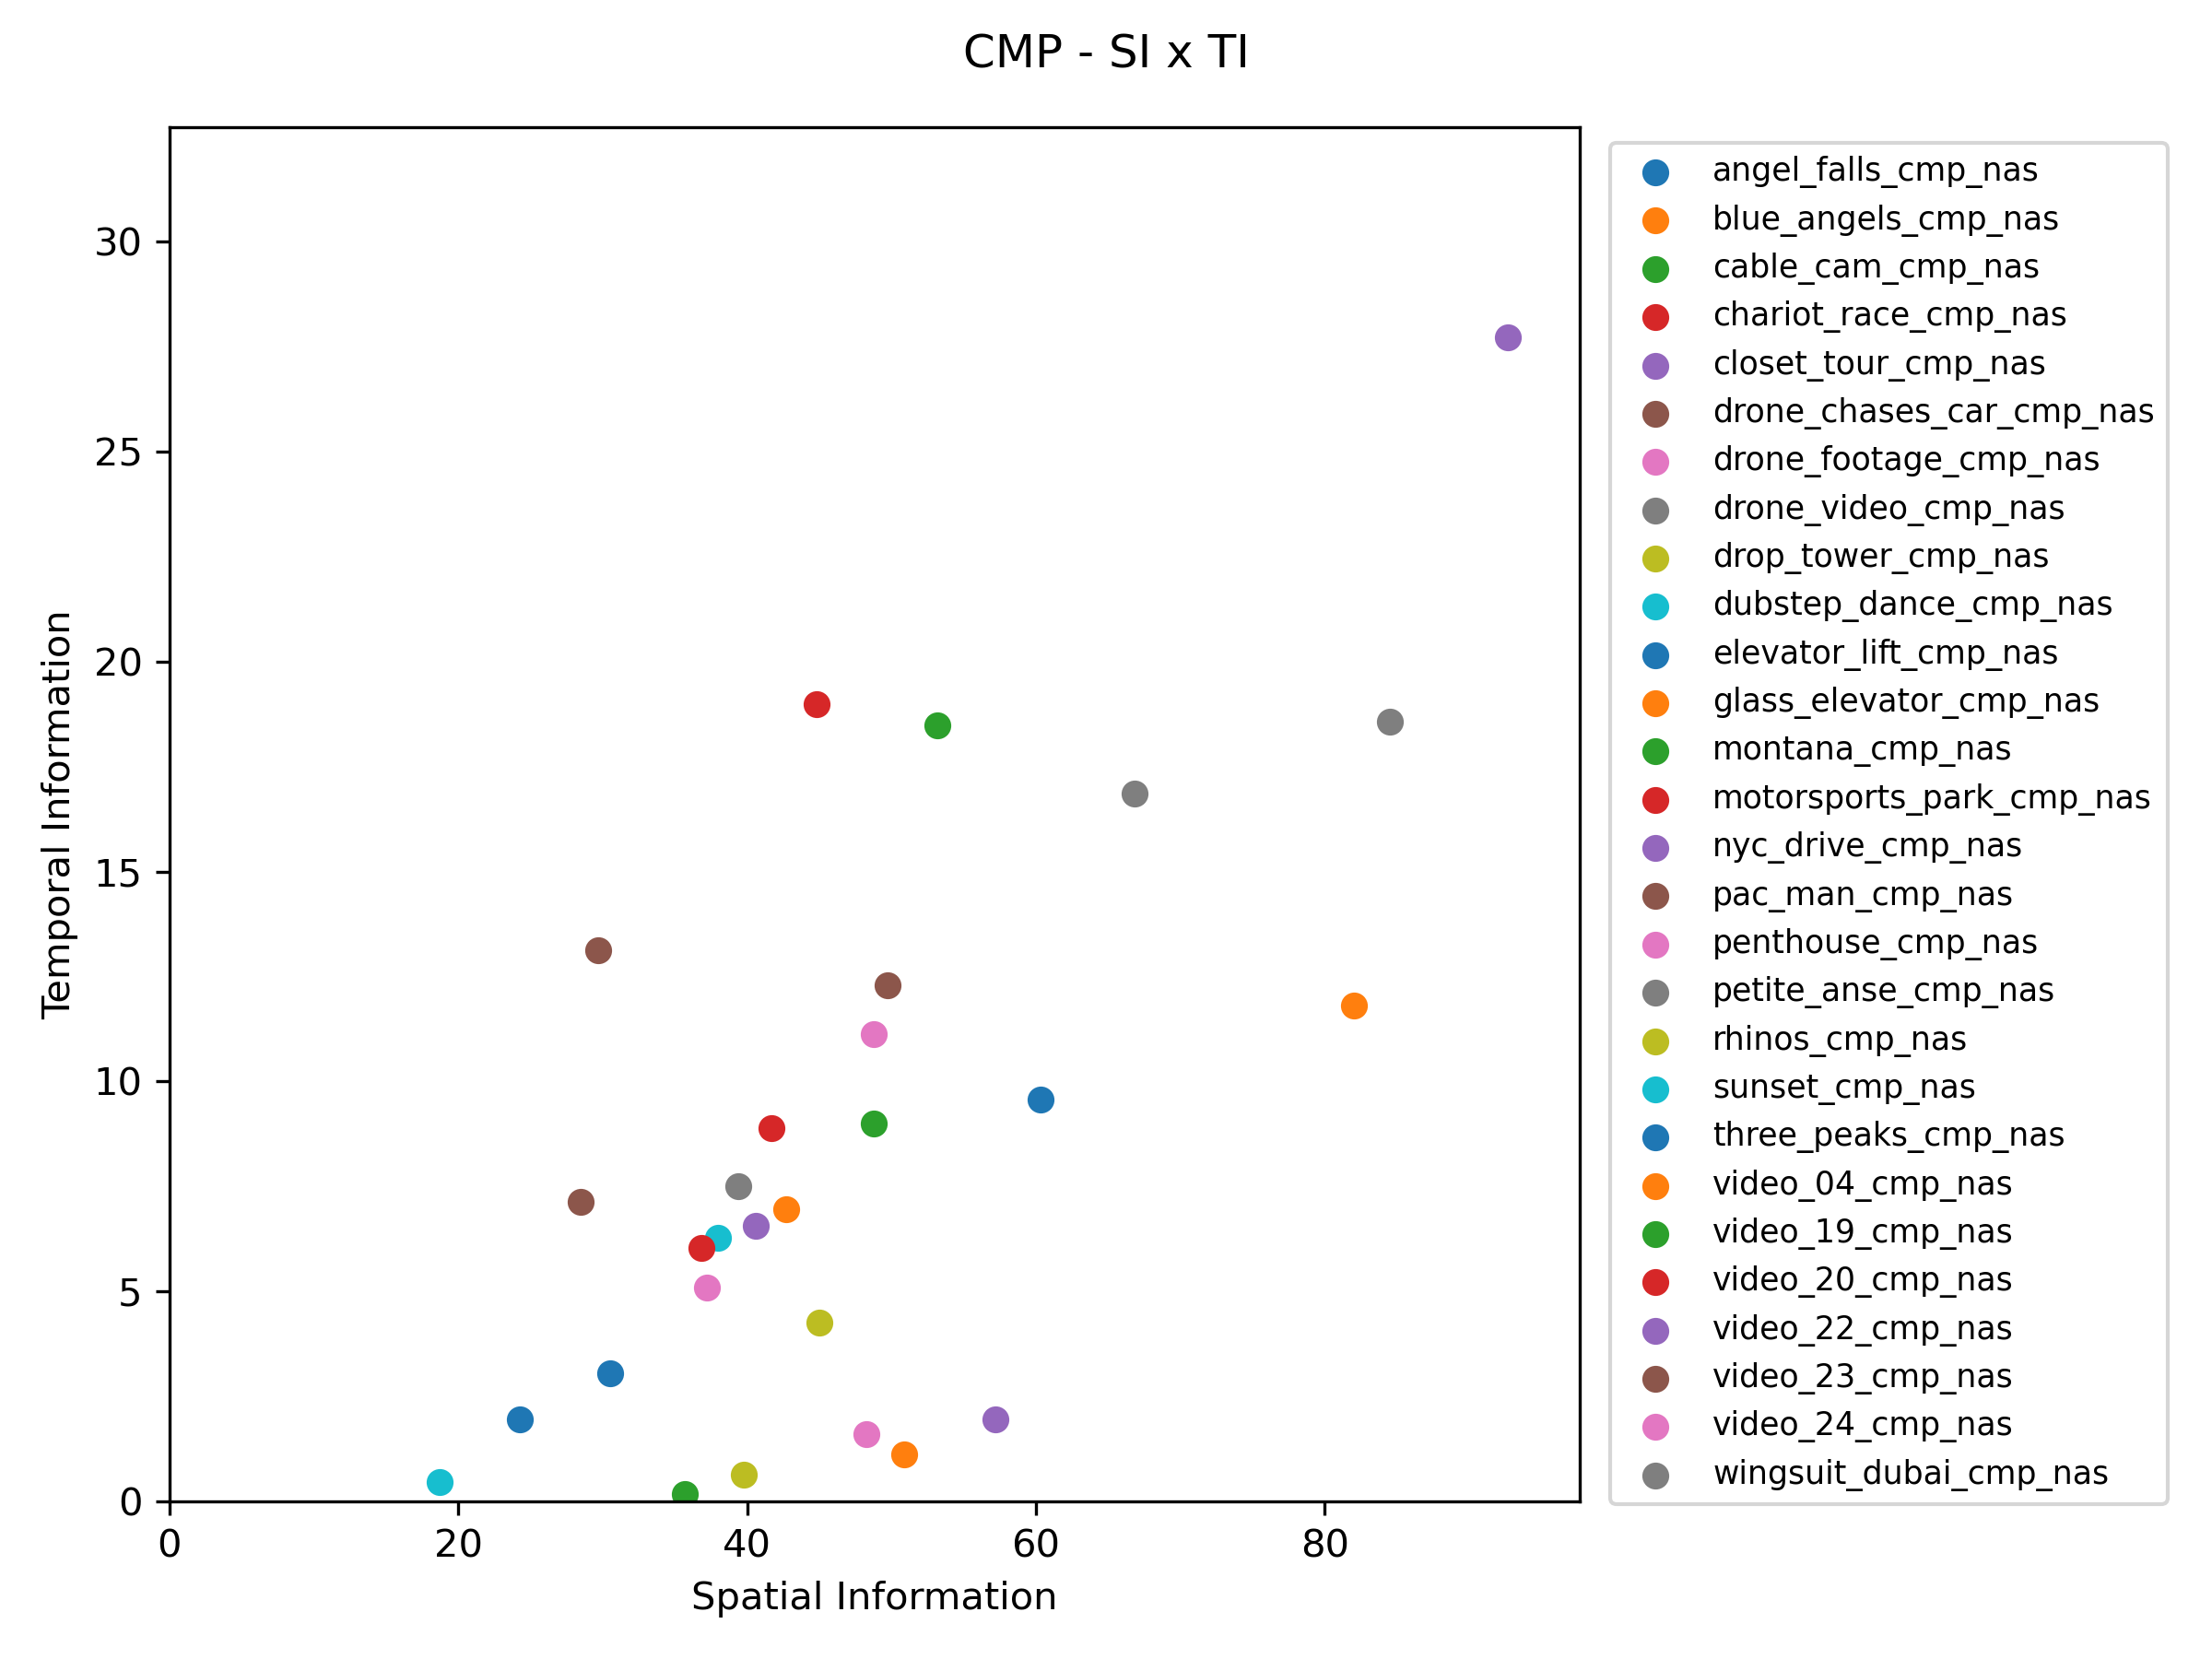
\includegraphics[width=0.45\linewidth]{fig/scatter_CMP.png}
} % end subfigure
\quad % dá um espaço entre as duas figuras.
\subfigure[Projeção ERP. \label{fig:scatter_ERP}]{
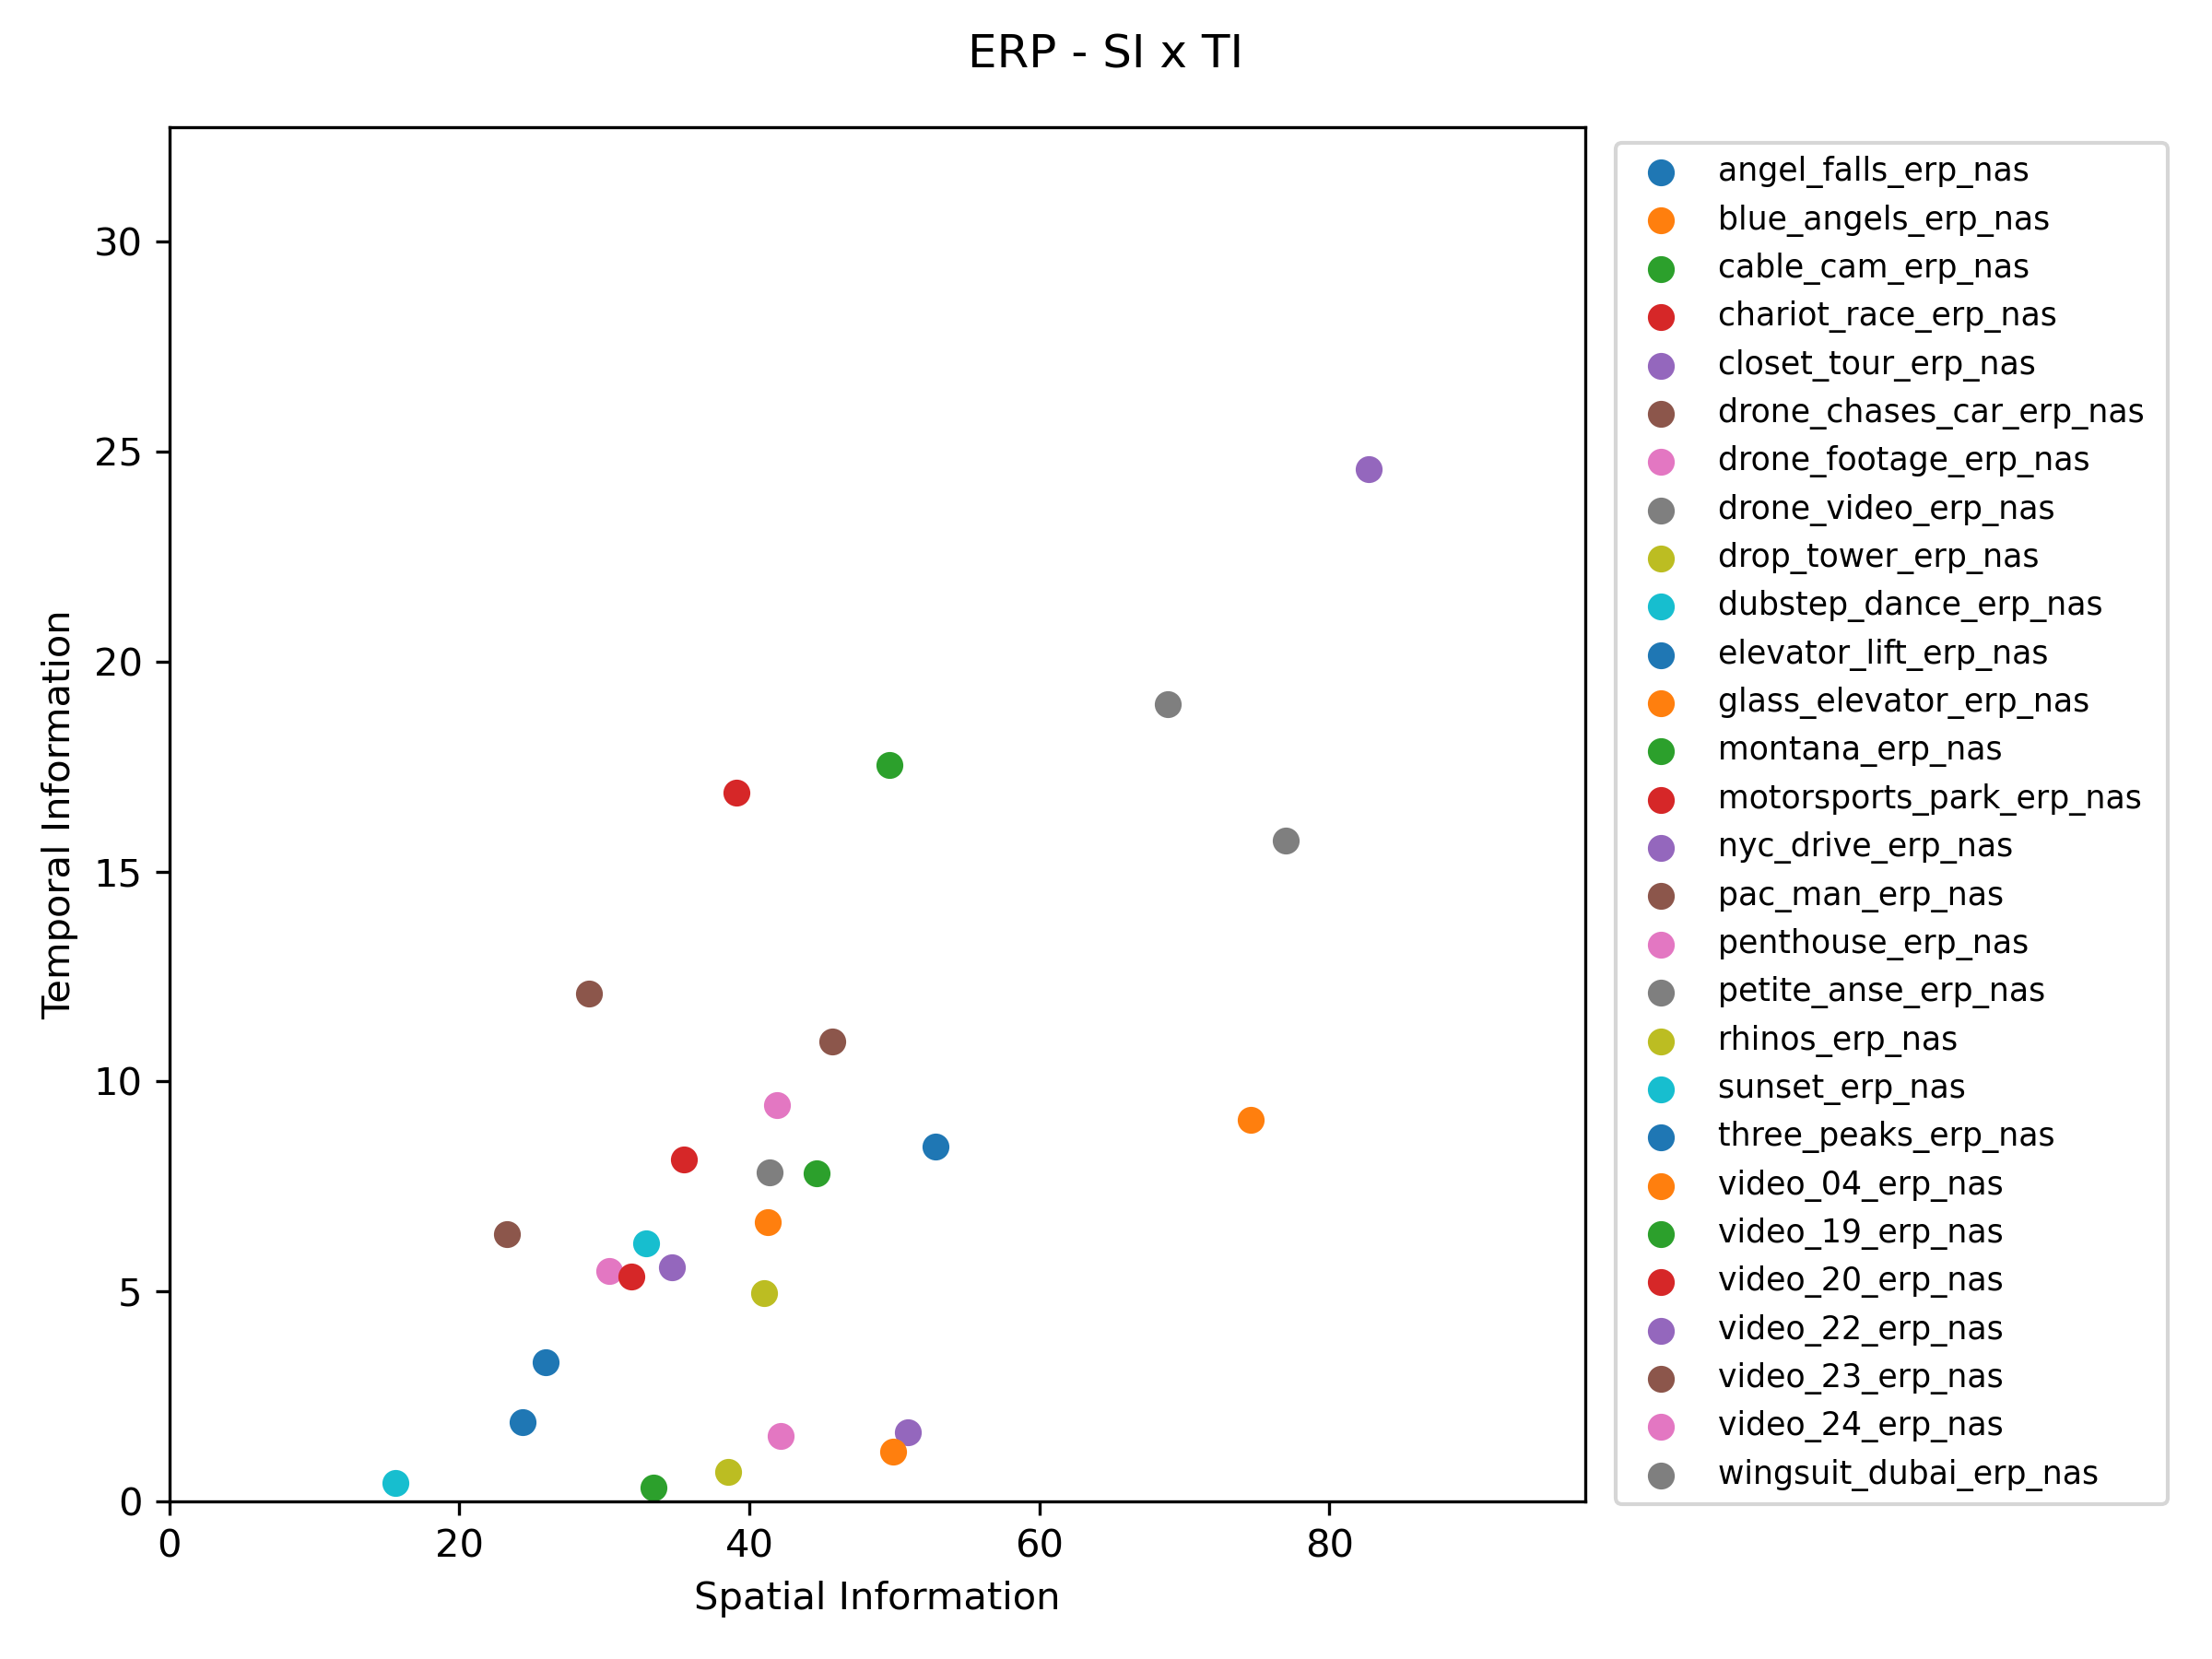
\includegraphics[width=0.45\linewidth]{fig/scatter_ERP.png}
} % end subfigure
\caption{Dispersão do SI e TI para as projeções avaliadas}
\label{fig:scatter_si_ti}
\end{figure}

Para replicar uma condição comparável DASH-SRD, os ladrilho passaram pelo ladrilhamento antes da codificação, garantindo que cada ladrilho fosse espacialmente independente. Para cada vídeo, geramos quatro novas sequências de vídeo, cada uma com padrões de os ladrilhos conforme a tabela~\ref{tab:ladrilhamento_resolucoes}. Quanto maior o numero de ladrilhos, menor o numero de pixel em cada ladrilho, reduzindo o espaço de busca do compensador de movimento do codificador e reduzindo a eficiência da compressão. A projeção cúbica, tendo proporção menor tende a ser uma representação mais compacta, apresentando menor taxa de bits, porém com maior complexidade de compressão. Apesar de quanto menor os ladrilhos, menos pixels não visto são processador, este procedimento produz redução na eficiência do codificador. Além disso, quanto mais ladrilhos forem solicitados, serão necessárias múltiplas instâncias de um decodificador no cliente e mais complexo será o processo, pois para reproduzir um único quadro do ladrilho, todo o chunk precisa ser decodificado.

\begin{table}[h]
    \centering
    \caption{Detalhes do ladrilhamento e resoluções resultantes.}
    \label{tab:ladrilhamento_resolucoes}
    \begin{tabular}{|c|p{2.5cm}|c|p{2.5cm}|c}
    \cline{1-4}
    \textbf{Ladrilhamento} & \centering\textbf{Quantidade de ladrilhos} & \textbf{Projeção} & \centering \textbf{Pixels por ladrilho} & \\ \cline{1-4}
    \multirow{2}{*}{\textbf{1x1}} & \centering\multirow{2}{*}{1} & CMP & \centering 4320x2160 & \\ \cline{3-4} 
        &   & ERP & \centering 3240x2160 & \\ \cline{1-4}
    \multirow{2}{*}{\textbf{3x2}} & \centering \multirow{2}{*}{6} & CMP & \centering 1440x1080 & \\ \cline{3-4} 
        &   & ERP & \centering 1080x1080 & \\ \cline{1-4}
    \multirow{2}{*}{\textbf{6x4}} & \centering \multirow{2}{*}{24} & CMP & \centering 720x540 & \\ \cline{3-4} 
        &   & ERP & \centering 540x540 & \\ \cline{1-4}
    \multirow{2}{*}{\textbf{9x6}} & \centering \multirow{2}{*}{54} & CMP & \centering 480x360 & \\ \cline{3-4} 
        &   & ERP & \centering 360x360  & \\ \cline{1-4}
    \multirow{2}{*}{\textbf{ 12x8}} & \centering \multirow{2}{*}{96} & CMP & \centering 360x270 & \\ \cline{3-4} 
         &    & ERP & \centering 270x270 & \\ \cline{1-4}
    \end{tabular}
\end{table}

Subsequentemente, utilizamos o codificador HEVC x265 no FFmpeg\footnote{https://ffmpeg.org/} para padronizar e codificar cada ladrilho, empregando seis valores distintos do Fator de Taxa Constante (CRF) para controlar a qualidade/taxa de bits: 16, 22, 28, 34, 40 e 46. O valor de CRF mais baixo (mais alto) de 16 (46) corresponde à maior (menor) qualidade de vídeo. O valor padrão de 28 é recomendado pelo codificador por seu equilíbrio entre qualidade e taxa de compressão. Vale ressaltar que cada incremento de 3 no valor de CRF resulta em uma redução pela metade na taxa de bits; em nosso conjunto, a taxa de bits diminui quatro vezes para os valores de CRF especificados. Os parâmetros de codificação do vídeo estão detalhados na Tabela \ref{tab:parametros_qlt}. O GOP do vídeo foi fixado em 30 quadros, o parâmetro para detecção de cortes de cena foi desativado para que o GOP não varie dentro de um chunk e o parâmetro "--no-info" foi utilizado para omitir cerca de 200 bytes de informações sobre o codificador no cabeçalho mp4 e assim reduzir o overhead dos vídeos. Esta quantidade é relativamente significativa quando se trata de chunks muito pequenos com baixa complexidade de codificação e alta compressão. Além disso os vídeos foram processados com os parâmetros "-tune psnr" para comparação mais precisa das métricas de distorção, como MSE e PSNR. 

\begin{table}[htb]
\centering
\footnotesize
\begin{tabular}{|l|c|}
    \hline
    \textbf{Resolução (Projeção)} & \makecell{$4320\times2160$ pixels (Cubemap), \\$3240\times2160$ pixels (Equirectangular)} \\ \hline
    \textbf{Taxa de Quadro} & 30 fps \\ \hline
    \textbf{GOP} & 30 quadros \\ \hline
    \textbf{Duração do Chunk} &  1 segundo \\ \hline
    \textbf{Qualidade (CRF)} & 0, 16, 22, 28, 34, 40 e 46 \\ \hline
    \textbf{Padrão de Ladrilho} & \makecell{$1\times 1$, $3 \times 2$, $6 \times 4$,  $9 \times 6$, $12\times 8$} \\ \hline
    \textbf{Codificador/Decodificador} & x265/FFmpeg 5.0-static \\ \hline
    \textbf{Configuração do x265} & keyint=30:min-keyint=30:open-gop=0:scenecut=0:info=0 \\ \hline
    \textbf{Sistema Operacional} & Ubuntu 22.04 \\ \hline
\end{tabular}
\caption{Parâmetros de codificação.}
\label{tab:parametros_qlt}
\end{table}

Após a codificação, usando o programa GPAC\footnote{https://github.com/gpac/gpac/}, cada ladrilho passou por uma segmentação temporal em fragmentos de 1 segundo, equivalentes a um GOP (Grupo de Quadros) completo de 30 quadros. Essa escolha considera que a previsão de movimento da cabeça tende a ser eficaz dentro de janelas de previsão de aproximadamente 1-2 segundos~\cite{Qian2016}. Subsequentemente, esses fragmentos foram encapsulados em um arquivo MP4 para facilitar a decodificação individual, acarretando em um overhead de cerca de 100-1000 bytes para incluir um cabeçalho MP4 adicional de "box moov" por fragmento. Apesar do overhead, esta abordagem permite a decodificação independente de cada chunk por qualquer tocador de vídeo. Desta forma, cada ladrilho de cada vídeo em cada projeção, compreende 60 fragmentos decodificáveis em seis qualidades diferentes, resultando em um total de 3.648.960 \textit{chunks} para análise.

O processo de decodificação de vídeo ocorreu em um computador desktop i7-4770 de 3,4 GHz equipado com 16 GB de RAM, rodando Linux Ubuntu 22.04. O decodificador nativo do FFmpeg foi utilizado, empregando apenas uma thread para a decodificação. As medidas de tempo de decodificação coletadas apresentam precisão de 1 ms e são relativas ao tempo de usuário (\textit{user time}), o que representa o tempo da CPU, excluindo operações do kernel como chamadas de sistema, focando especificamente em tarefas de decodificação, como operações matriciais, por exemplo. Cada fragmento de um dado ladrilho passou por decodificação cinco vezes para produzir um tempo médio de decodificação. Devido a natureza multiprocesso e da hierarquia de memória, foi possível observar uma variação do tempo de decodificação de até 93,75\%. Além disso, medimos a taxa de bits de cada \textit{chunk} simplesmente multiplicando o tamanho do arquivo por oito, já que cada \textit{chunk} possui exatamente 1 segundo.

A seguir, para cada quadro de cada chunk, métricas objetivas de qualidade, incluindo SSIM, MSE, WS-MSE e S-MSE, serão calculadas comparando os quadros decodificados os vídeos codificados com CRF 0. As métricas são armazenadas em um JSON em uma estrutura de árvores, em que cada nível representa respectivamente a projeção, nome do video, padrão de ladrilhamento, crf, ladrilho e chunk. No caso do tempo de decodificação, foi armazenado um valor para cada decodificação.

Para a análise das distribuições estatística dos chunks codificados, empregamos a biblioteca Python SciPy. Por padrão, a SciPy utiliza do método de Estimação por Máxima Verossimilhança para determinar os parâmetros da distribuições de probabilidade de densidade (PDF). As distribuições analisadas são: Burr Tipo XII , Birnbaum-Saunders, Gamma, Inversa Gaussiana, Rayleigh, Log Normal, Generalized Pareto, Pareto, Half-Normal, e Exponencial\footnote{https://docs.scipy.org/doc/scipy/reference/stats.html}. Como ferramenta auxiliar foi utilizado o pacote Fitter para testar todas as distribuições\footnote{https://fitter.readthedocs.io/}. Além das distribuições foi analisada a correlação entre as métricas e para a avaliação dos erros, foi utiliza a raiz do erro quadrático médio (RMSE). Nos resultados produzidos pela Scipy, os valores são normalizados e os parâmetros de deslocamento ({\it loc}) e escala ({\it scale}) devem ser aplicados à distribuição normalizada para obter a ajustada, conforme a equação~\ref{eq:shift_scale}.

\begin{equation}
\label{eq:shift_scale}
\text{fitted\_pdf}(x) = \left( \frac{1}{scale} \right) \text{normalized\_pdf}\left(\frac{x-loc}{scale}\right).
\end{equation}


\section{Caracterização dos elementos do cliente}

% kd o diagrama?
Para a caracterização do que o usuário experimenta, a posição da cabeça do usuário é utilizada para identificar as ladrilhos necessárias para a reconstrução da viewport. Foi desenvolvido uma bibliteca para conversão de coordenadas na esfera e um mecanismo para seleção de ladrilhos com base na posição da cabeça do usuário. Este mecanismo foi implementado em Python, e, quando fornecido o padrão de ladrilhamento, dimensões da projeção e posição da viewport, ele retorna uma lista de ladrilhos que estão visíveis na viewport. Existem vários métodos para selecionar e priorizar ladrilhos~\cite{Nguyen2020}. Porém, neste trabalho, focamos em considerar apenas os ladrilhos visíveis, essenciais para a construção da viewport, conforme ilustrado na Figura~\ref{fig:tilesSelection}. Este mecanismo foi aplicado com um banco de dados de posição da cabeça do usuário para calcular uma lista de ladrilhos que aparecem na viewport durante a reprodução.

\begin{figure}[htb]
    \centering
    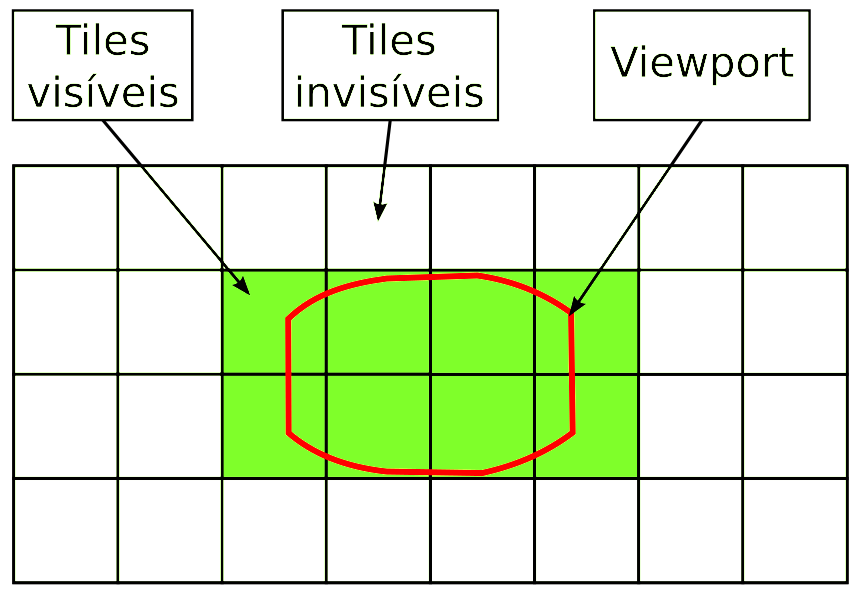
\includegraphics[width=0.6\linewidth]{fig/tiles selection simples.png}
    \caption{Mecanismo para seleção de ladrilhos.}
    \label{fig:tilesSelection}
\end{figure}

O banco de dados de movimentos da cabeça foi gerado por Nasrabadi \cite{Nasrabadi2019}. Este banco de dados compilou a posição central do viewport na esfera para 60 voluntários (30 voluntários por vídeo), representados em quatérnions e em vetores cartesianos a uma taxa variável. Utilizando marcas de tempo foi feita a interpolação para que todas as amostras estejam à taxa de 30 Hz. A figura \ref{fig:datasetSpeedmap}, extraída do trabalho de Nasrabadi, fornece um mapa da velocidade angular média para todos os usuários em cada vídeo. Como observado pelo autor, a velocidade angular média dos vídeos depende do usuário, o que significa que um usuário com velocidade alta em um vídeo tende a exibir velocidade alta em todos os vídeos. 

\begin{figure}
    \centering
    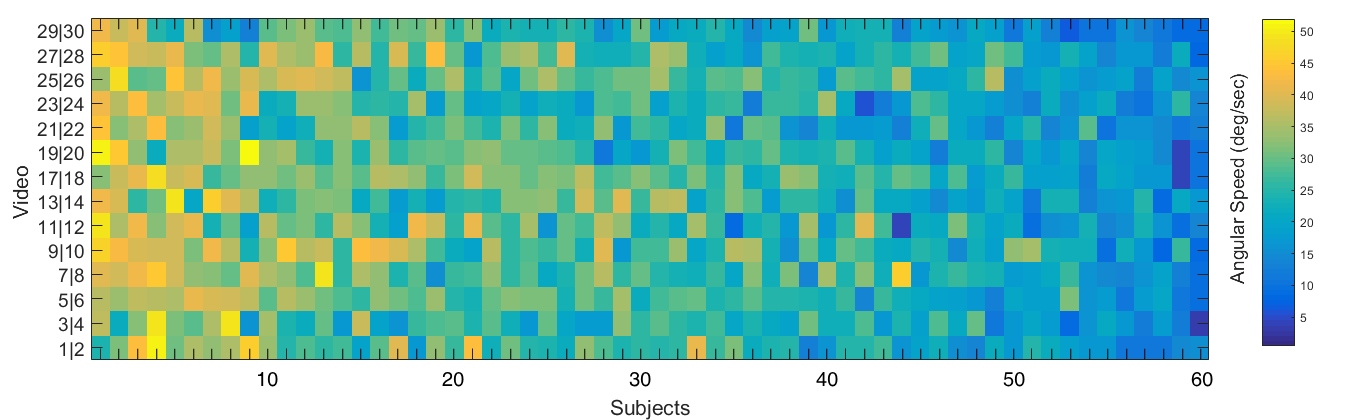
\includegraphics[width=0.8\linewidth]{fig/datasetSpeedmap.png}
    \caption{Mapa da velocidade angular média de todos os voluntários para todos os grupos de vídeo. Extraído de  \cite{Nasrabadi2019}}
    \label{fig:datasetSpeedmap}
\end{figure}

A seguir, considerando os ladrilhos selecionados na etapa anterior, são reconstruídos a projeção e geradas viewports tanto de vídeos não compactados (CRF 0) quanto de vídeos codificados com qualidade variável para uma mesma região, com base nas regiões que os indivíduos visualizaram anteriormente. nas regiões da projeção que o ladrilho não foi selecionado é preenchido com zero. A criação da viewport é realizada utilizando a projeção Gnomônica (chamada também de projeção retilinear) restrita pelo campo de visão (FOV) do dispositivo. Nossa janela de visualização é configurada com um FOV horizontal e vertical de 100°x90°, um valor aproximado daqueles adotados pela linha Oculus Quest~\footnote{https://risa2000.github.io/hmdgdb/}. A seguir, será calculado o PSNR entre o quadro da viewport criado com ladrilhos compactados e o quadro da viewport criado com ladrilhos não compactados (com CRF 0).


\section{Cenários avaliados}

Após a coleta dos dados, o comportamento da qualidade será analisado sob duas perspectivas: uma do ponto de vista de um sistema ABR que considera a correlação da qualidade com a taxa de transmissão do vídeo e outra do ponto de vista do usuário que visualiza o vídeo utilizando óculos de realidade virtual. 

\subsection{Estatísticas por ladrilhos}

A tabela~\ref{tab:stats} fornece os valores de média e desvio padrão para o tempo de decodificação e a taxa de bits dos \textit{chunk} para vários padrões de ladrilho. Além disso, também foi incluído o coeficiente de correlação entre essas medidas. Conforme previsto, a redução no tamanho do ladrilho (correspondendo a um aumento na segmentação do ladrilho) está correlacionada com uma diminuição no tempo de decodificação do ladrilho e na taxa de bits do ladrilho. Além disso, o desvio padrão, em relação ao valor médio, aumenta à medida que o tamanho do bloco diminui, com um impacto mais pronunciado na taxa de bits do que no tempo de decodificação.

Vale ressaltar que a faixa considerada de valores CRF (16 a 46) resulta em uma variação substancial de aproximadamente 20 vezes na taxa de bits. Examinar a correlação entre o tempo de decodificação e a taxa de bits em todos os níveis de qualidade revela uma associação moderada, e essa associação diminui com a diminuição do tamanho do bloco. Esta redução indica que o 

\begin{longtable}{|c|c|c|c|c|c|}
    \caption{Os valores médios e de desvio padrão para o tempo de decodificação do bloco e a taxa de bits do bloco são apresentados de acordo com os padrões de ladrilhamento, abrangendo todos os níveis de qualidade.} \label{tab:stats} \\

    \hline
    \multirow{2}{*}{\textbf{Métrica}} &  \multirow{2}{*}{\textbf{Ladrilhamento}} & \multicolumn{2}{c|}{\textbf{CMP}} & \multicolumn{2}{c|}{\textbf{ERP}} \\
    \cline{3-6}
                            &   & \textbf{Média} & \textbf{Desvio Padrão} & \textbf{Média} & \textbf{Desvio Padrão} \\
    \hline
    \endfirsthead

    \multicolumn{6}{c}%
    {{\bfseries \tablename\ \thetable{} -- Continuação da página anterior}} \\
    \hline
    \endhead
    
    \hline \multicolumn{6}{|r|}{{Continua na próxima página}} \\ \hline
    \endfoot
    
    \hline
    \endlastfoot

    \multirow{5}{*}{Taxa}  & 1x1  & 6.050.720 & 10.352.018 & 6.591.315 & 11.176.695 \\ \cline{2-6}
                            & 3x2  & 1.030.891 & 2.012.731  & 1.130.073 & 2.281.468 \\ \cline{2-6}
                            & 6x4  & 277.689   & 589.369    & 301.493   & 661.050  \\  \cline{2-6}
                            & 9x6  & 133.972   & 273.547    & 144.640   & 318.278  \\  \cline{2-6}
                            & 12x8 & 84.727    & 163.725    & 90.798    & 188.049  \\   \hline
    \multirow{5}{*}{Tempo} & 1x1  & 0,629     & 0,278      & 0,757     & 0,311     \\  \cline{2-6}
                            & 3x2  & 0,098     & 0,053      & 0,122     & 0,062    \\  \cline{2-6}
                            & 6x4  & 0,022     & 0,015      & 0,026     & 0,017    \\  \cline{2-6}
                            & 9x6  & 0,011     & 0,007      & 0,012     & 0,008    \\  \cline{2-6}
                            & 12x8 & 0,006     & 0,004      & 0,008     & 0,005    \\  \hline 
% \pagebreak\hline
    \multirow{5}{*}{MSE}   & 1x1  & 21,472    & 33,788     & 17,782    & 28,024    \\  \cline{2-6}          
                            & 3x2  & 21,603    & 39,575     & 18,155    & 34,290   \\  \cline{2-6}
                            & 6x4  & 21,923    & 45,121     & 18,409    & 39,623   \\  \cline{2-6}
                            & 9x6  & 22,523    & 48,846     & 18,853    & 43,182   \\  \cline{2-6}
                            & 12x8 & 22,613    & 50,499     & 19,034    & 45,037   \\  \hline 
    \multirow{5}{*}{SSIM}  & 1x1  & 0,951     & 0,050      & 0,957     & 0,043     \\  \cline{2-6}
                            & 3x2  & 0,951     & 0,060      & 0,957     & 0,055    \\  \cline{2-6}
                            & 6x4  & 0,951     & 0,068      & 0,957     & 0,061    \\  \cline{2-6}
                            & 9x6  & 0,951     & 0,071      & 0,957     & 0,064    \\  \cline{2-6}
                            & 12x8 & 0,951     & 0,073      & 0,957     & 0,067    \\  \hline 
    \multirow{5}{*}{WS-MSE}& 1x1  & 21,784    & 33,965     & 20,473    & 33,051   \\  \cline{2-6}
                            & 3x2  & 21,968    & 40,410     & 20,880    & 39,442   \\  \cline{2-6}
                            & 6x4  & 22,420    & 45,615     & 19,578    & 42,162   \\  \cline{2-6}           
                            & 9x6  & 22,738    & 49,216     & 19,401    & 44,243   \\  \cline{2-6}                
                            & 12x8 & 22,758    & 50,740     & 19,343    & 45,660   \\  \hline 
    \multirow{5}{*}{S-MSE}  & 1x1  & 21,779    & 34,009     & 20,461    & 33,072   \\  \cline{2-6}
                            & 3x2  & 3,661     & 6,749      & 3,477     & 6,572    \\  \cline{2-6}
                            & 6x4  & 0,935     & 1,904      & 0,883     & 2,084    \\  \cline{2-6}
                            & 9x6  & 0,427     & 0,963      & 0,401     & 1,014    \\  \cline{2-6}
                            & 12x8 & 0,241     & 0,568      & 0,228     & 0,597 
\end{longtable}

A Figura ~\ref{Figura:histograma-fmt} descreve, para cada padrão de ladrilho, as três melhores funções de densidade de probabilidade ajustadas à distribuição empírica do tempo de decodificação do ladrilho. A partir dos resultados, a distribuição Log-Normal está entre as três distribuições mais bem ajustadas em 100\% dos padrões, enquanto as distribuições Gaussiana Inversa e Birnbaum-Saunders aparecem em 87,5\% e 75\% dos casos, respectivamente.

% \begin{figure*}[htb]
% \centering
%   \includegraphics[width=2\columnwidth]{fig/hist_30bins_tudo_crf.png}
%   \caption{Funções de densidade de probabilidade ajustadas aos tempos de decodificação de ladrilhos medidos de acordo com o padrão de ladrilhos. Este caso considera-se chunks com todos os níveis de qualidade.}
%   \label{Figure:histogram-fmt}
% \end{figure*}

%%%%%%%%%%%
%% Statistic By Quality
%%%%%%%%%%%
\subsection{Estatísticas por nível de qualidade e ladrilhamento}

%Corrigir estes valores
A Figura ~\ref{Figura:bar-fmt-qlt} ilustra o tempo médio de decodificação do ladrilho e a taxa de bits média por nível de qualidade para cada padrão de ladrilho. A redução na taxa de bits correspondente a uma diminuição na qualidade do vídeo é acompanhada por uma diminuição semelhante, embora menos pronunciada, no tempo de decodificação dos blocos. Por exemplo, no cenário $6 \times 4$, onde a taxa de bits diminui em 97,5\% (de 1,91 Mbps para 47,6 Kbps) em uma faixa CRF de 16 a 46, o tempo de decodificação do bloco diminui apenas 63,1\% (de 0,067 a 0,025 segundos) para a mesma faixa CRF.

Analisando os resultados, fica evidente que as três distribuições mais bem ajustadas variam de acordo com o padrão de ladrilho. As frequências com que aparecem entre os três primeiros são as seguintes: Birnbaum-Saunders (79,2\%), Gaussiana Inversa (72,9\%), Log-Normal (70,8\%), Burr Tipo XII (41,7\%), Gama (8,33\%), Pareto Generalizado (8,3\%), Half Normal (6,3\%), Exponencial (3,08\%) e Rayleigh (2,1\%).

% \begin{figure*}[hbt]
% \centering
%   \includegraphics[width=2\columnwidth]{fig/bar_fmt-quality_30bins_crf.png}
%   \caption{Tempo médio de decodificação para blocos (representado por barras azuis) e taxa de bits média (representada por linhas vermelhas) categorizados por padrão de ladrilho e nível de qualidade do ladrilho.}
%   \label{Figure:bar-fmt-qlt}
% \end{figure*}

Tabela~\ref{tab:corr_list} fornece os resultados da correlação entre o tempo de decodificação do bloco e a taxa de bits média em todos os casos. Notavelmente, para um determinado padrão de ladrilhos, a correlação tende a aumentar com níveis de qualidade mais elevados. Por outro lado, para um determinado valor de CRF, a correlação diminui à medida que o número de blocos por quadro aumenta.

Como ilustração, considerando o padrão de ladrilhos de $6 \times 3$, a correlação é de aproximadamente 0,728 para CRF = 28. É digno de nota que esse padrão de ladrilhos específico demonstrou alcançar economias substanciais de largura de banda em pesquisas anteriores~\cite{Graf2017}.

\begin{table}[htb]
\footnotesize
\caption{Correlação entre o tempo de decodificação do bloco e a taxa de bits do bloco.}
\label{tab:corr_list}
\begin{center}
\begin{tabular}{|c|c|c|c|c|c|c|}
    \hline
    \multirow{2}{*}{\textbf{Padrão}} & \multicolumn{6}{c|}{\bf Qualidade (CRF)} \\
    \cline{2-7}
      & \textbf{16} & \textbf{22} & \textbf{28} & \textbf{34} & \textbf{40} & \textbf{46} \\
    \hline
    $1\times 1$ & 0.893 & 0.839 & 0.803 & 0.786 & 0.704 & 0.554 \\
    \hline
    $3\times 2$ & 0.857 & 0.781 & 0.735 & 0.684 & 0.610 & 0.479 \\
    \hline
    $4\times 3$ & 0.846 & 0.782 & 0.744 & 0.674 & 0.584 & 0.497 \\
    \hline
    $6\times 3$ & 0.848 & 0.788 & 0.734 & 0.683 & 0.581 & 0.471 \\
    \hline
    $6\times 4$ & 0.843 & 0.789 & 0.728 & 0.673 & 0.566 & 0.451 \\
    \hline
    $6\times 5$ & 0.827 & 0.761 & 0.703 & 0.636 & 0.537 & 0.424 \\
    \hline
    $6\times 6$ & 0.814 & 0.748 & 0.687 & 0.617 & 0.520 & 0.403 \\
    \hline
    $7\times 6$ & 0.808 & 0.743 & 0.688 & 0.605 & 0.505 & 0.398 \\
    \hline
\end{tabular}
\end{center}
\end{table}

%%%%%%%%%%%
%% Full-Frame Statistic
%%%%%%%%%%%
\subsection{Estatísticas dos \textit{Chunks} para o envio de todos o ladrilhos}

Agora, nosso foco muda para o tempo necessário para decodificar sequencialmente todos os ladrilhos de um intervalo de tempo, considerando todos os vídeos e níveis de qualidade coletivamente. Desta forma poderemos simular o pior caso, onde o usuário terá que solicitar e processar toda a esfera. A Figura~\ref{Figura:bar-fmt} ilustra o tempo médio de decodificação do pedaço e a taxa de bits média para cada padrão de ladrilho, com barras de erro indicando o desvio padrão.

Como previsto, a taxa de bits apresenta um aumento correspondente ao aumento no número de blocos por quadro. Este resultado é atribuído ao fato de que a segmentação de blocos restringe o espaço de busca para a previsão de movimento do codificador. Inesperadamente, o tempo médio de decodificação do bloco se beneficia da segmentação lado a lado, com valores médios geralmente menores que aqueles observados para o caso $1 \times 1$. Observa-se que o tempo médio de decodificação diminui à medida que o número de ladrilhos por quadro aumenta, atingindo um mínimo no ladrilhamento $6 \times 3$. Esse mínimo é aproximadamente 10,8\% menor que o padrão $1 \times 1$, e essa melhoria é alcançada com apenas um aumento de 6,26\% na taxa de bits. Além deste ponto, os valores do tempo de decodificação começam a subir novamente. As razões específicas por trás deste comportamento merecem uma investigação mais aprofundada, pois a complexidade do vídeo codificado reduz a medida que os ladrilhos diminuem de tamanho, tornando mais rápido a decodificação do conjunto, porém o número de bits aumenta, o que aumentaria o tempo de decodificação. Contudo, a exploração desta ocorrência está além do escopo deste trabalho.

% \begin{figure}[htb]
%     \centering
%     \includegraphics[width=0.8\columnwidth]{fig/bar_fmt-dectime_x_time_ts.png}
%     \caption{Tempo de decodificação de pedaços e taxa de bits média por padrão de ladrilho.}
%     \label{Figure:bar-fmt}
% \end{figure}

Nossas medições revelam uma correlação significativa entre o tempo médio de decodificação do chunk e sua taxa de bits média em todos os padrões de ladrilhos. O coeficiente de correlação medido ultrapassa 0,96 em todos os casos. A Figura~\ref{Figura:hist-somafmt} ilustra as três distribuições de probabilidade com menor erro para os dados coletados em cada padrão de ladrilho.

Notavelmente, as distribuições Gaussiana Inversa e Birnbaum-Saunders estão consistentemente classificadas entre as três primeiras em 100\% dos padrões, enquanto a distribuição Log-Normal aparece entre as três primeiras em 87,5\% dos padrões. A distribuição Burr Tipo XVII surge como uma candidata potencial para o caso $1 \times 1$. Infelizmente, os valores específicos dos parâmetros de distribuição para este caso não são apresentados devido a limitações de espaço.

% \begin{figure*}[htb]
% 	\centering
% 	\includegraphics[width=2\columnwidth]{fig/hist_60bins_fmt_somatiles_crf.png}
% 	\caption{O histograma de densidade do tempo de decodificação para todos os padrões de blocos e as três melhores distribuições com o RMSE menor, para o vídeo em blocos completo.}
% 	\label{Figure:hist-somafmt}
% \end{figure*}




\subsection{Ladrilhos vistos (por viewport)}

No primeiro cenário, para cada chunk haverá um conjunto de ladrilhos que aparecem no viewport. Ao longo da duração do chunk o usuário poderá mover a cabeça e o conjunto de ladrilhos muda. Estes novos ladrilhos precisam já ter sido decodificados completamente para poderem ser exibidos. Desta forma é preciso considerar a trajetória do movimento de cabeça para se requisitar os ladrilhos. Sendo A o conjunto dos ladrilhos que são vistos pelo viewport no quadro f, os ladrilhos vistos $lv$ durante a duração de um chunk será dada pela equação~\ref{eq:tiles_seen}.

\begin{equation}
    lv=\bigcup^{30}_{f=1} A_f \\    
    \label{eq:tiles_seen}
\end{equation}

A taxa de bits de $lv$ será igual a soma da taxa de todos os ladrilhos de $lv$. Para o tempo de decodificação de $lv$, podemos ter duas abordagens. Decodificação em série: os ladrilhos de $lv$ são decodificados em série e o tempo total de decodificação de todos será igual a soma do tempo de todos os ladrilhos de $lv$. A segunda abordagem é a decodificação em paralelo: Neste caso o tempo de decodificação de $lv$ é definido pelo maior tempo de todos os ladrilhos de $lv$. Já a qualidade, devemos considerar a média do MSE, SSIM, S-MSE e WS-MSE de todos os ladrilhos em $lv$. Por fim, uma seção de vídeo $sv$ consiste de uma sequencia de $lv$ com tamanho igual ao numero de chunks de um vídeo. Em $sv$ temos todos os ladrilhos que foram vistos ao longo do vídeo separados em blocos de 1 segundo. Cada ladrilho tem associado sua posição espacial e temporal, indicada por um índice na lista de ladrilhos e pelo número do chunk que foi visto ao longo da reprodução. Como temos 30 usuários por vídeo, 28 vídeos, dois tipos de projeção e cinco tipos de ladrilhamento, teremos ao todo 8400 seções que podem ser reproduzidas considerando seis qualidades. Entre as métricas avaliadas, estão o número de ladrilhos utilizados pelo viewport ao longo da reprodução, taxa de bits, tempo de decodificação e qualidade do viewport e dos ladrilhos na projeção. Essa análise também pode ser estendida para diversas técnicas de seleção de ladrilho.

% \section{Resultados}
